\documentclass{article}
\usepackage[utf8]{inputenc}
\usepackage{polski}
\usepackage{amsmath}
\usepackage{anysize}
\usepackage[pdftex]{graphicx}
\marginsize{2,5cm}{2,5cm}{1cm}{4cm}
\begin{document}

Wiktor Zuba 320501 grupa 4
\newline

Zad.1.
\newline
\newline
Narysować izokliny i naszkicować krzywe całkowe równania
$
x(\frac{dx}{dt}+1)=1
$\newline
$
\dot{x}=\frac{1}{x}-t
$
izokliny
$
x=\frac{1}{t+k}
$\newline
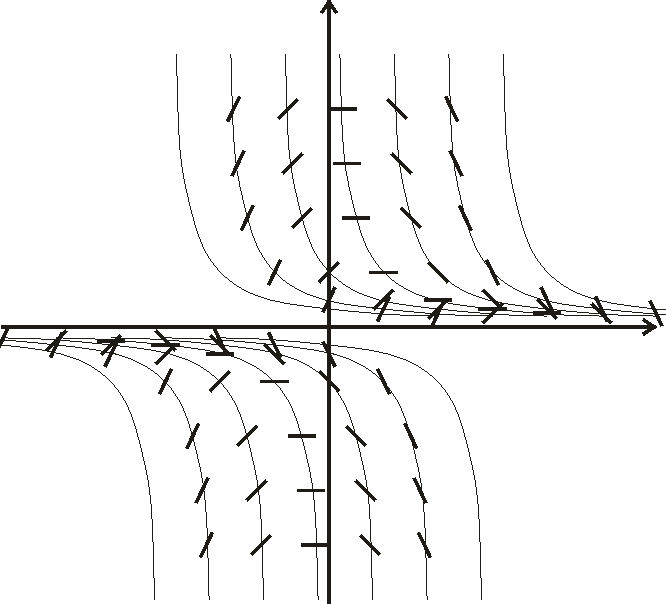
\includegraphics[scale=0.75]{hiperbole2.png}
\newline\newline


Zad.2.
\newline
\newline
Rozwiązanie zagadnienia Cauchy'ego
$
(t+2x)\dot{x}=1,x(0)=-1
$\newline
Jako, że rówanie nie daje się zbyt łatwo zaklasyfikować w jeden z poznanych typów równań
łatwiej może być znaleźć rozwiązanie szczególne, a następnie udowodnienie jego jednoznaczności\newline
Próba znalezienia rozwiązania liniowego:
$
x=at+b\quad 
\left\{\begin{array}{cc}
(t+2at+2b)a=1\\b=-1\\
\end{array}\right.
\quad
\left\{\begin{array}{cc}
2ta^2+(t-2)a-1=0\\b=-1\\
\end{array}\right.
$
\newline
$
\left\{\begin{array}{cc}
a=\frac{1}{t}\\b=-1\\
\end{array}\right.
\quad\vee\quad
\left\{\begin{array}{cc}
a=-\frac{t}{2}\\b=-1\\
\end{array}\right.
$
bierzemy drugą możliwość
$
\underline{x=-\frac{t}{2}-1}
$\newline
Jednoznaczność:
$
\dot{x}=\frac{1}{2x+t}
$
Jak w twierdzeniu Picarda-Lindel$\ddot{o}$fa $Q=\{(t,x):|t-t_0|\le\frac{1}{2},|x-x_0|\le\frac{1}{2}\}$
dla $t_0=0,x_0=-1$ mamy $\sup|f(t,x)|=2$ jako że $2x+t$ jest odgrodzone od 0 (mniejsze niż $-\frac{1}{2}$), to spełnia warunek Lipshitza
tak więc z twierdzenia wynika, że dla $|t-t_0|\le\alpha<min(\frac{1}{2},\frac{1}{4})=\frac{1}{4}$ rozwiązanie jest jednoznaczne, możemy teraz zamiast 
$t_0=0$ wziąść $t_0=\frac{\alpha}{2}(x_0=-1-\frac{\alpha}{4})$, lub $t_0=-\frac{\alpha}{2}(x_0=-1+\frac{\alpha}{4})$,
dla których powyższe równości przy tych samych ograniczeniach zostają prawdziwe (dokładnie te same stałe), tak więc skoro o takie $\frac{\alpha}{2}$
możemy przesunąć dowolnie wiele razy to rozwiązanie jest jednoznaczne globalnie.
\newpage

Wiktor Zuba 320501 grupa 4
\newline


Zad.3.
\newline
\newline
Wszystkie krzywe całkowe równania
$
(2x+y-4ln(y))dy=ydx\quad y>0$ bo tylko dla takich  ma sens$ln(y)\newline
\frac{2x(y)+y-4ln(y)}{y}=x'(y)\quad x'-\frac{2}{y}x=1-\frac{4ln(y)}{y}\newline
$Równanie Liniowe-metoda czynnika całkującego:
$
e^{-2ln(y)}x'-\frac{2}{y}e^{-2ln(y)}x=(1-\frac{4ln(y)}{y})e^{-2ln(y)}
\newline
\frac{x'}{y^2}-\frac{2x}{y^3}=\frac{1}{y^2}-\frac{4ln(y)}{y^3}
\quad
(\frac{x}{y^2})'=\frac{1}{y^2}-\frac{4ln(y)}{y^3}
$\newline
Całkując stronami:($-\frac{4ln(y)}{y^3}$ przez części)
$
\frac{x}{y^2}=-\frac{1}{y}+\frac{2ln(y)+1}{y^2}+c
\quad
\underline{x=-y+2ln(y)+1+cy^2}
$
\newline
\newline

Zad.4.
\newline
\newline
Rozwiązanie ogólne $xy'+2y+x^5e^xy^3=0$\newline
$
$(dla $x=0\Rightarrow y=0), \quad $dla $x\neq0\quad y'+\frac{2}{x}y=-x^4e^xy^3
$
Równanie Bernoulliego-podstawienie $z=y^{-2} (*)$
$
\frac{y'}{y^3}+\frac{2}{x}y^{-2}=-x^4e^x
\quad -\frac{1}{2}z'+\frac{2}{x}z=-x^4e^x
\quad z'-\frac{4}{x}z=2x^4e^x
$\newline
Równanie liniowe-metodą czynnika całkującego\quad
$
z'e^{-4ln(x)}-\frac{4}{x}e^{-4ln(x)}z=2x^4e^xe^{-4ln(x)}
\quad x^{-4}z'-\frac{4}{x}x^{-4}z=2e^x
\quad (zx^{-4})'=2e^x
$\newline
Całkując obie strony
$
zx^{-4}=2e^x+c
\quad
z=(2e^x+c)x^4
$\newline
Co nie przyjmuje wartości $\pm\infty$ dla żadnych x a 0 tylko dla $x=0$ - który to przypadek został już rozważony osobno, co uprawomacnia przejście (*)\newline
$
\underline{y=\frac{1}{x^2\sqrt{e^x+c}}\quad\vee\quad y=\frac{-1}{x^2\sqrt{e^x+c}}}
$
\newline
\newline

Zad.5.
\newline
\newline
Wszystkie krzywe całkowe równania
$
(x^2-\sin{(y)}^2)dx+(x\sin{(2y)})dy=0
\newline
M(x,y)=x^2-\sin{(y)}^2,
N(x,y)=x\sin{(2y)}
\quad
M_y=-sin(2y)=-N_x
$\newline
Nierówne więc poprzez czynnik całkujący ($x\neq 0$,dla $x=0\Rightarrow x'=0\Rightarrow x=c$, z $y$ tak samo)
$
f(x)=\frac{1}{xsin(2y)}(-2sin(2y))=\frac{-2}{x}\quad
\mu(x)=e^{\int\frac{-2}{x}}=x^{-2}
\quad
(1-\frac{sin(y)^2}{x^2})dx+\frac{sin(2y)}{x}dy=0
$\newline
Równanie w postaci różniczki zupełnej:
$
F(x,y)=\int\frac{sin(2y)}{x}dy+c(x)=\frac{sin(y)^2}{x}+c(x)
\quad
1-\frac{sin(y)^2}{x^2}=-\frac{sin(y)^2}{x^2}+c'(x)\Rightarrow c(x)=x+c_2
\quad
F(x,y)=\frac{sin(y)^2}{x}+x+c_2
$\newline
Odwikłując
$
x^2+c_3x+sin(y)^2=0
\quad
x=\frac{-c_3\pm\sqrt{c_3^2-4sin(y)^2}}{2}=\underline{\frac{c\pm\sqrt{c^2-4sin(y)^2}}{2}}
$




\end{document}
